%\documentclass[]{beamer}
\documentclass[handout]{beamer}
%\documentclass[handout,draft]{beamer}

% Preambulo
% Paquetes para usar bien el idioma español
\usepackage[spanish,es-tabla]{babel}
\selectlanguage{spanish}
\usepackage[utf8]{inputenc}

% Paquetes para usar mejores imagenes
\usepackage{graphicx}

% Paquetes para links y tabla de contenidos en el PDF
\usepackage{hyperref}
\hypersetup{colorlinks=true,allcolors=blue}
%\usepackage{hypcap}

% Paquetes para mejores tablas
\usepackage{booktabs}

% Mejor matematica
\usepackage{amsmath}

% Fuentes de las imagenes
\usepackage[absolute,overlay]{textpos}

% Paquete captions
\usepackage[justification=centering,labelformat=empty,labelsep=none]{caption}

% Opciones para ticks
\usepackage{tikz}
\usetikzlibrary{shapes,arrows,positioning}

\tikzstyle{decision} = [diamond, draw, fill=blue!20, text width=4em, text badly centered, node distance=2cm, inner sep=0pt,on grid]
\tikzstyle{block} = [rectangle, draw, fill=blue!20, text width=8em, text centered, rounded corners, minimum height=2em,on grid]
\tikzstyle{line} = [draw, -latex]

% Citas bibliograficas
\usepackage[backend=biber]{biblatex}
\renewcommand{\footnotesize}{\tiny}
\addbibresource{biblio.bib}

% Mejoro las captions
\setbeamertemplate{caption}{\raggedright\insertcaption\par}

\setbeamertemplate{caption}{%
\begin{beamercolorbox}[wd=0.85\paperwidth, sep=.2ex]{block body}\insertcaption%
\end{beamercolorbox}%
}


% Sacar barra de navegacion
\setbeamertemplate{navigation symbols}{}%remove navigation symbols

% Transparencias en items
\setbeamercovered{transparent}

% Estilo de diapositivas
% \usetheme{Boadilla}
\usecolortheme{whale}
\usecolortheme{orchid}


\title{Herramientas de Teledetección Cuantitativa\\{\small Clase 4}}
\author{Francisco Nemi\~na}
\institute{Unidad de Educación y Formación Masiva \\ ComisiÓn Nacional de
Actividades Espaciales}
%\institute[Inst.]{
\includegraphics[height=1cm]{Figures/logosopi.png}\phantom{pepe} 
\includegraphics[height=1cm]{Figures/2mp.png}\phantom{pepe} 
\includegraphics[height=1cm]{Figures/conae.png}}
\date{}
%\titlegraphic{
%\includegraphics[height=1cm]{IMAGENES/minplan.png}\phantom{1}
%
\includegraphics[height=1cm]{IMAGENES/conae.png}\phantom{1}
%
\includegraphics[height=1cm]{IMAGENES/sopi.png}}

\logo{
\includegraphics[height=0.7cm]{imagenes/sopi.png}}

\AtBeginSection[]
{
\begin{frame}
\frametitle{Esquema de presentación}
\tableofcontents[currentsection]
\end{frame}
}


\begin{document}
\begin{frame}
    \maketitle
\end{frame}

\section{Transformaciones}
\subsection{Motivación}

\begin{frame}{Motivación}
  \begin{center}
      \resizebox{0.4 \linewidth}{!}{%
        \begin{tikzpicture}[node distance = 2cm, auto]
          \node[block]                                (init) {Firma Espectral};\pause
          \node[block, below= of init]                (resp) {Reflectancia Espectral Efectiva};
          \path[line] (init) --          (resp);
          \pause
          \node[decision, below= of resp]             (ques) {????};
          \path[line] (resp) --          (ques);\pause
        \end{tikzpicture}%
      }%
    \end{center}
\end{frame}
%--- Next Frame ---%

\begin{frame}{Motivación}
  \begin{block}{Técnicas de reducción de la dimensionalidad}
    \begin{itemize}[<+>]
      \item Rotaciones
      \item \'Indices
      \item Clasificaciones
    \end{itemize}
    \pause
    Empezamos con las primeras dos.
  \end{block}
\end{frame}
%--- Next Frame ---%

\subsection{Matemática}


\begin{frame}{Matemática}
  \begin{block}{Definición:}
    Un vector es un objeto de la forma $$\left(
    \begin{array}{c}
          v_1 \\
          \vdots \\
          v_n
        \end{array}
        \right) $$.
  \end{block}\pause
  \begin{block}{Propiedades}
    Con dos operaciones
    $$ \begin{array}{c} v+w \\ \alpha v \end{array}  $$
    \pause
    y viven en un lugar que se llama espacio vectoral
  \end{block}
\end{frame}
%--- Next Frame ---%

\begin{frame}{Matemática}
  \begin{block}{Definición:}
    Las matrices se pueden pensar como transformaciones que convierten a un vector en otro. \pause
    $$ Av = w$$
  \end{block}\pause
  \begin{alertblock}{Propiedad}
    Como las transformaciones que utilizaremos son lineales, con sólo definirlas en unos pocos valores alcanza. \pause Elegir bien los vectores para definir la transformación es útil.
  \end{alertblock}
\end{frame}
%--- Next Frame ---%

\begin{frame}{Matemática}
  \begin{figure}
    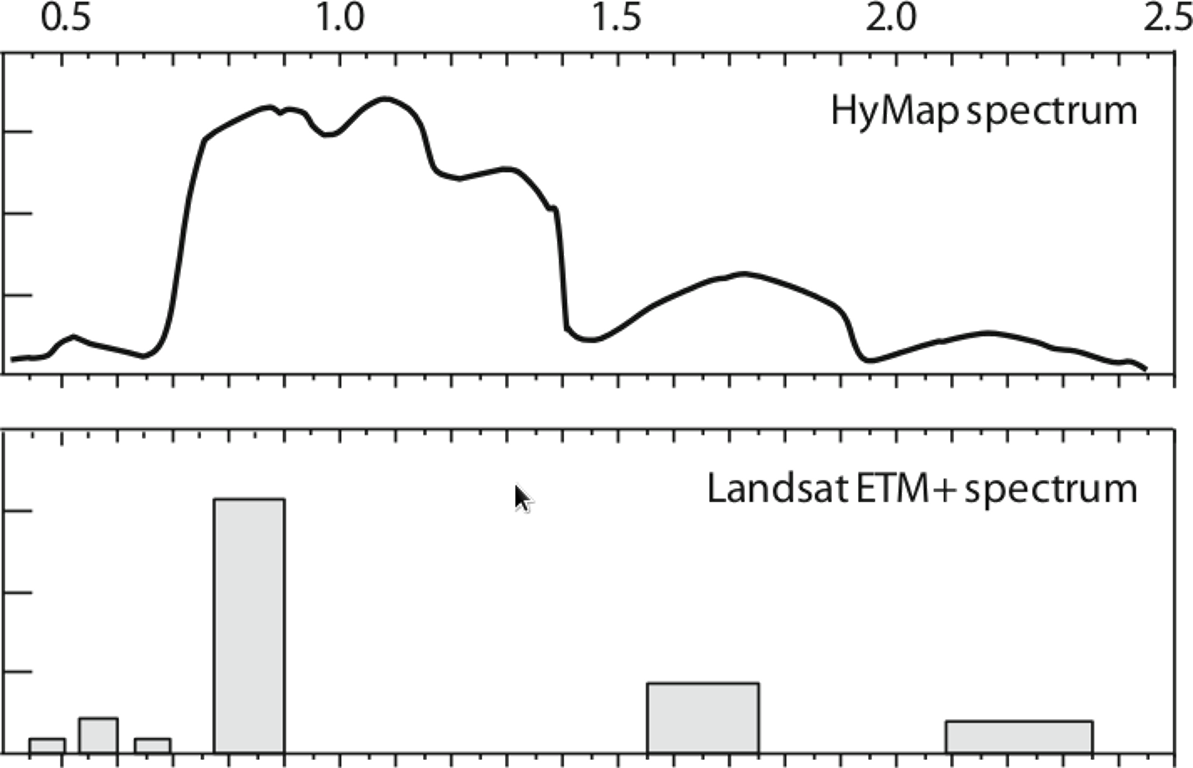
\includegraphics[width=0.6\textwidth]{imagenes/elandsat.png}
    \caption{Comparación entre firma espectral y valores medidos para un píxel\footfullcite{richards2013remote}}
  \end{figure}
\end{frame}
%--- Next Frame ---%

\begin{frame}{Matemática}
  \begin{figure}
    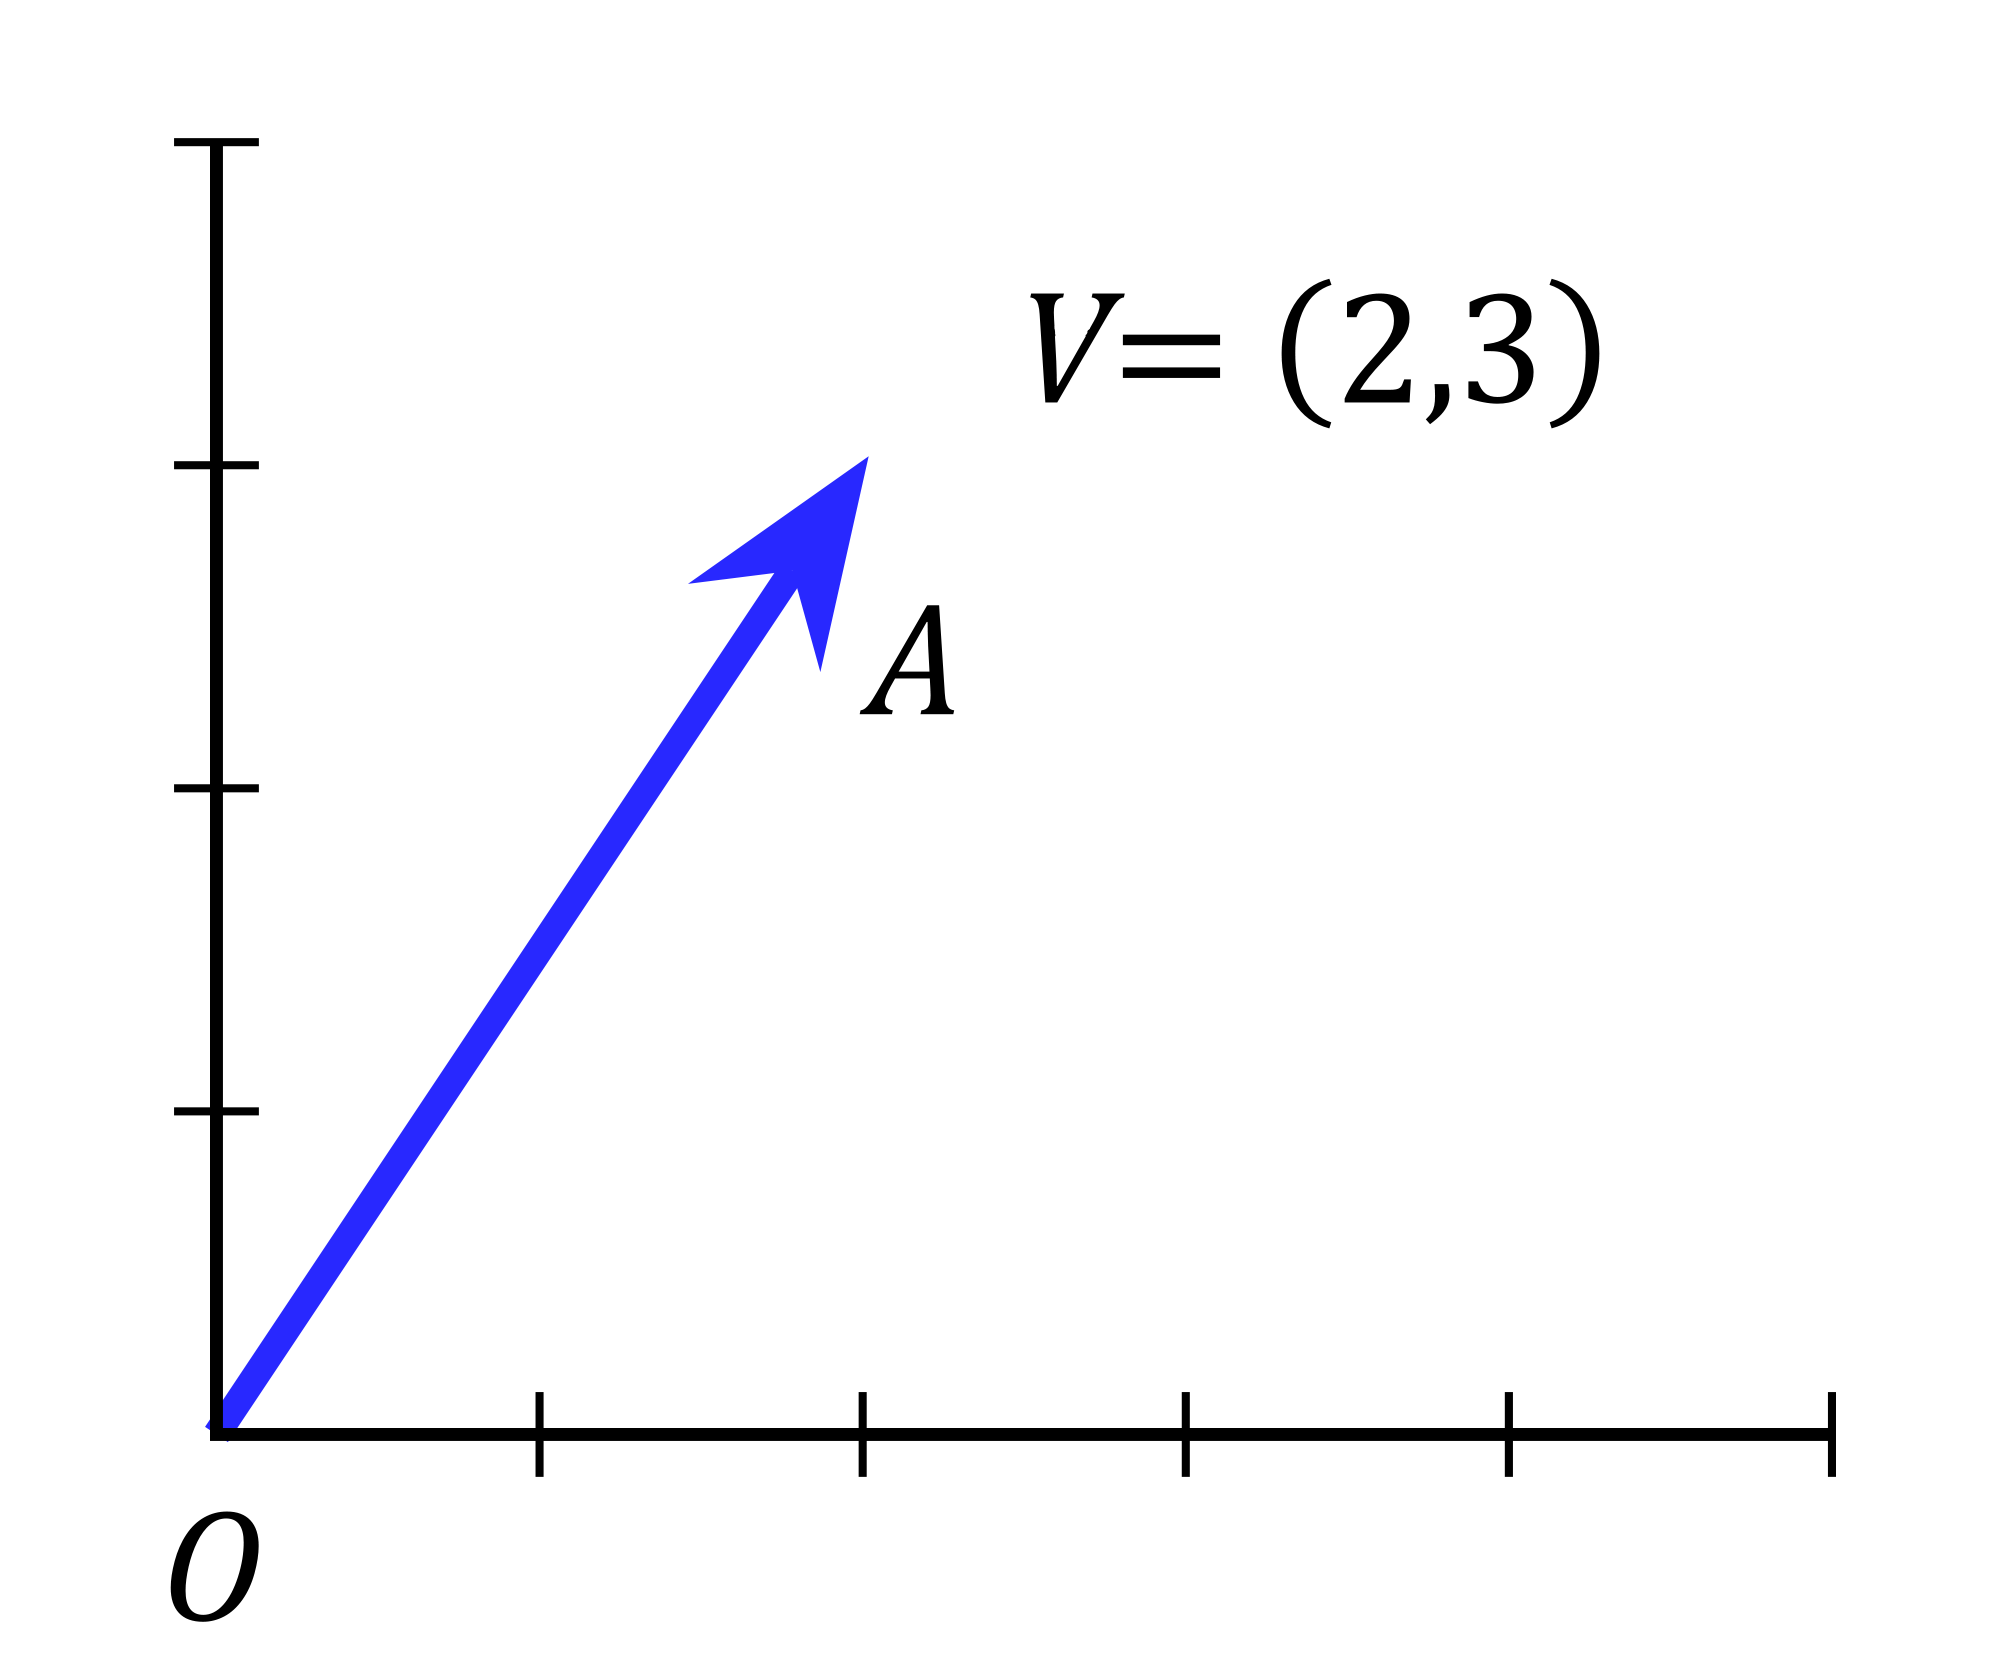
\includegraphics[width=0.6\textwidth]{imagenes/vector.png}
    \caption{Píxeles en $R^2$.\footfullcite{richards2013remote}}
  \end{figure}
\end{frame}
%--- Next Frame ---%

\begin{frame}{Matemática}
  \begin{alertblock}{Respuesta efectiva como vector}
    A la respuesta espectral efectiva la puedo pensar como un vector de reflectancias
    $$\left(
    \begin{array}{c}
          \rho_1 \\
          \vdots \\
          \rho_n
        \end{array}
    \right) $$.
  \end{alertblock}
  \pause
\end{frame}
\begin{frame}{Matemática}
  \begin{exampleblock}{Ejemplo:}
    $$v_{(x,y)}=\left(
    \begin{array}{c}
      0.03 \\
      0.08 \\
      0.04 \\
      0.40 \\
      0.20 \\
      0.15
    \end{array}
    \right) ,
    a_{(x,y)}=\left(
    \begin{array}{c}
      0.05 \\
      0.03 \\
      0.01 \\
      0.01 \\
      0.00 \\
      0.00
    \end{array}
    \right) ,
    s_{(x,y)}=\left(
    \begin{array}{c}
      0.08 \\
      0.10 \\
      0.15 \\
      0.20 \\
      0.25 \\
      0.30
    \end{array}
    \right) $$
  \end{exampleblock}
\end{frame}
%--- Next Frame ---%

\begin{frame}{Matemática}
  \begin{alertblock}{Motivación}
    Podemos pensar a una imagen como vectores en un espacio vectorial. El número de bandas es la dimensión de ese espacio.
  \end{alertblock}
\end{frame}
%--- Next Frame ---%

\section{Rotaciones}
\subsection{Idea}
\begin{frame}{Idea}
  Empecemos con un ejemplo para una imagen de dos bandas
  \begin{figure}
  \centering
  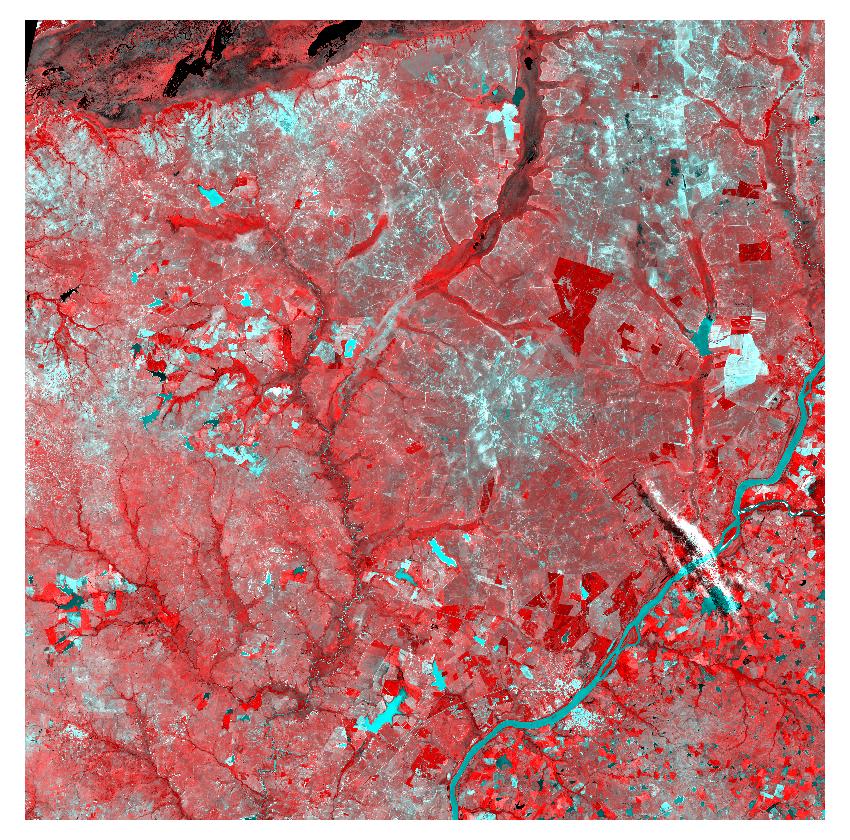
\includegraphics[width=0.6\textwidth]{imagenes/nir-red.png}
  \caption{Imagen de dos bandas.}
  \end{figure}
\end{frame}
%--- Next Frame ---%

\begin{frame}{Idea}
  \begin{figure}
  \centering
  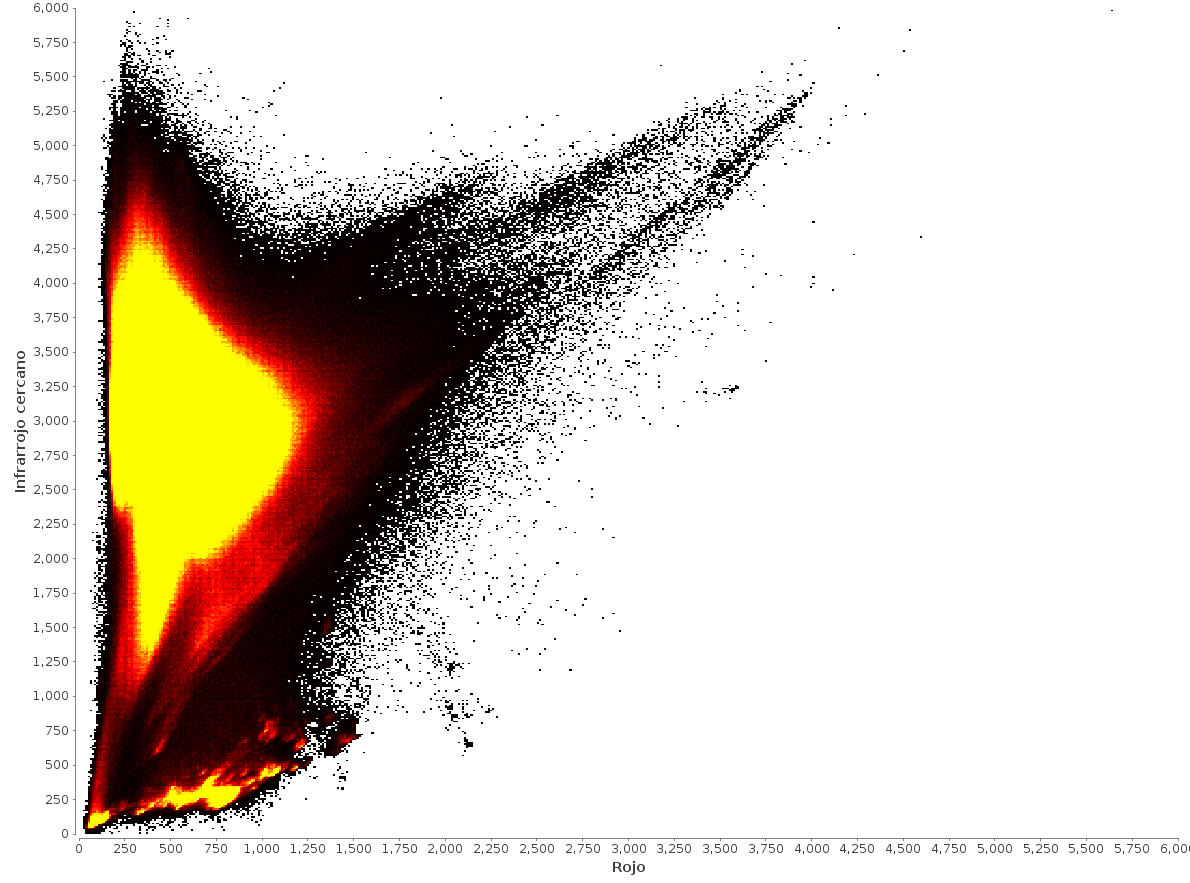
\includegraphics[width=0.8\textwidth]{imagenes/nir-red2.png}
  \caption{Imagen de dos bandas en el espacio vectorial.}
  \end{figure}
\end{frame}
%--- Next Frame ---%

\begin{frame}{Idea}
  \begin{alertblock}{Transformación}
    Una combinación obvia es $$ DIF = 0.5NIR-0.5RED$$
    y
    $$ SUM = 0.5NIR+0.5RED $$
  \end{alertblock}
\end{frame}
%--- Next Frame ---%


\begin{frame}{Idea}
  \begin{alertblock}{Importante}
    No siempre más bandas significa mas información.
  \end{alertblock}
\end{frame}
%--- Next Frame ---%

\subsection{Componentes principales}

\begin{frame}{Componentes principales}
  \begin{block}{Idea}
    Queremos ver si un set bandas está correlacionadas o no.
  \end{block}
\end{frame}
%--- Next Frame ---%

\begin{frame}{Componentes principales}
  \begin{figure}
  \centering
  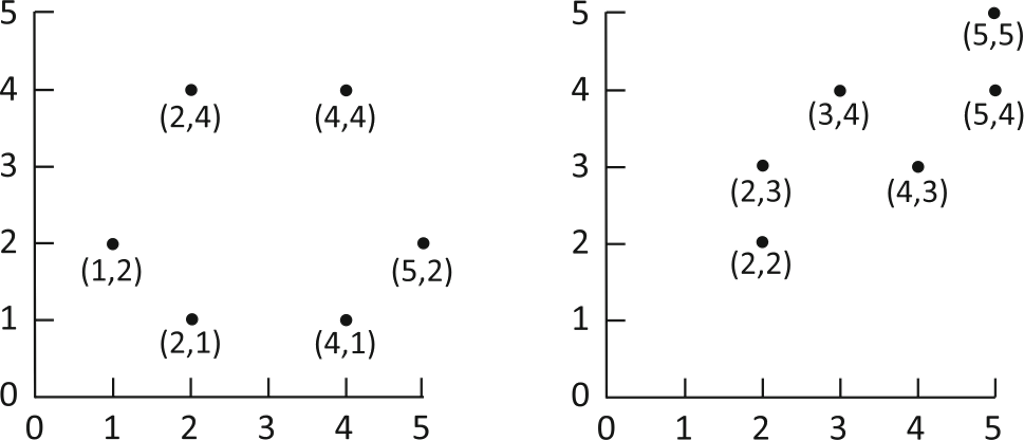
\includegraphics[width=0.8\textwidth]{imagenes/corr.png}
  \caption{Datos correlacionados y no correlacionados\footfullcite{richards2013remote}}
  \end{figure}
\end{frame}
%--- Next Frame ---%



\begin{frame}{Componentes principales}
  \begin{block}{Matriz de correlación}
    Tiene en sus componentes las funciones de correlación entre cada banda\pause
    \[
    A = \begin{bmatrix}
        corr_{11}       & corr_{12} & corr_{13} & \dots & corr_{1n} \\
        corr_{21}       & corr_{22} & corr_{23} & \dots & corr_{2n} \\
        \vdots          & \vdots    & \vdots    & \ddots & \vdots \\
        corr_{n1}       & corr_{d2} & corr_{n3} & \dots & corr_{nn}
    \end{bmatrix} \]
  \end{block}
\end{frame}
%--- Next Frame ---%

\begin{frame}{Componentes principales}
  \begin{block}{Observaciones}
      Queremos que la correlación cruzada entre bandas sea cero. \pause Matemáticamente lo pedimos como
        $$Av=\lambda v$$
      Y nos quedamos como vectores útiles a los que cumplan esto.
  \end{block}
\end{frame}
%--- Next Frame ---%

\begin{frame}{Componentes principales}
  \begin{block}{Matriz de correlación}
    La forma de la matriz va a depender de las combinaciones lineal que haga entre los vectores \pause
    \[
    \begin{bmatrix}
        \lambda{1}       & 0 & 0 & \dots & 0 \\
        0       & \lambda_{2} & 0 & \dots & 0 \\
        \vdots & \vdots & \vdots & \ddots & \vdots \\
        0       & 0 & 0 & \dots & \lambda_{n}
    \end{bmatrix} \]
    \pause
    donde son los autovectores $$\lambda_{1}  > \lambda_{2} > \dots > \lambda_{n}$$
  \end{block}
\end{frame}
%--- Next Frame ---%

\begin{frame}{Componentes principales}
  \begin{block}{Observaciones}
    \begin{itemize}[<+>]
      \item $\frac{\lambda_i}{\sum_i \lambda_i}$ me habla de cuanto me explica ese vector sobre la variabilidad de la imagen
      \item $(v_1 , \dots , v_n)$ el autovector que me representa la combinación de bandas de un autovalor dado.
      \item Estas combinación lineal de bandas tienen la información más relevante.
    \end{itemize}
  \end{block}
\end{frame}
%--- Next Frame ---%

\begin{frame}{Componentes principales}
  \begin{exampleblock}{Ejemplo}
    Volviendo al ejemplo de antes
    \[
    \begin{bmatrix}
        1       & 0.329127 \\
        0.329127 & 1
    \end{bmatrix} \]
  \end{exampleblock}
\end{frame}
%--- Next Frame ---%

\begin{frame}{Componentes principales}
  \begin{exampleblock}{Ejemplo}
    Al diagonalizar me queda
    \[
    \begin{bmatrix}
        1.343685       & 0 \\
        0       & 0.656315
    \end{bmatrix} \]
    con autovectores $$0.707107\, NIR-0.707107 \, RED$$  y $$0.707107 \, NIR+0.707107\, RED$$ \pause
    Acá el primer vector explica el el 67\% de la variabilidad de la imagen y el segundo del 33\%.
  \end{exampleblock}
\end{frame}
%--- Next Frame ---%

\begin{frame}{Componentes principales}
  \begin{figure}
  \centering
  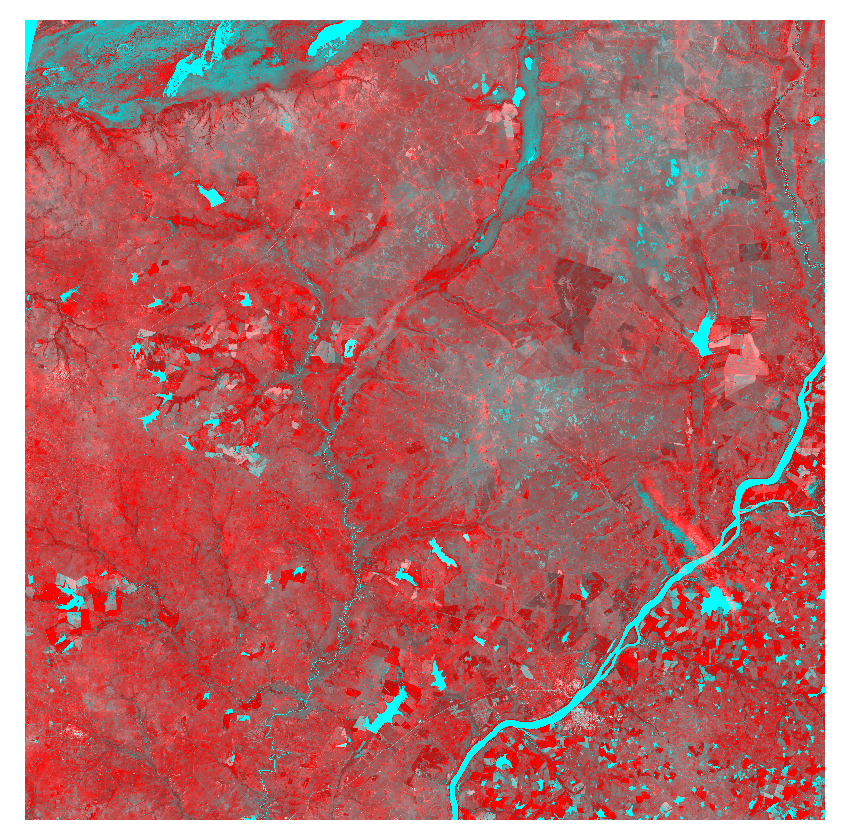
\includegraphics[width=0.6\textwidth]{imagenes/pca1.png}
  \caption{Ejemplo con las bandas NIR-RED en la imagen.}
  \end{figure}
\end{frame}
%--- Next Frame ---%

\begin{frame}{Componentes principales}
  \begin{figure}
  \centering
  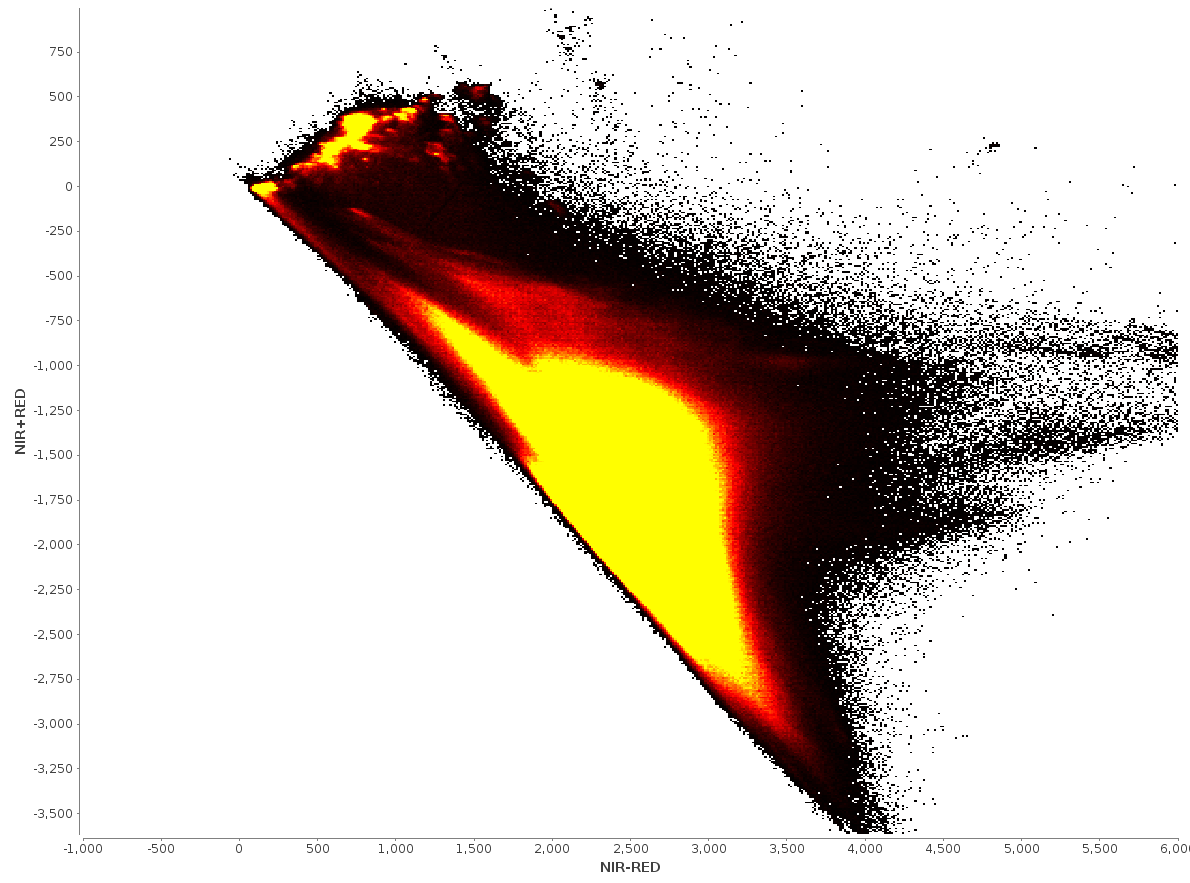
\includegraphics[width=0.8\textwidth]{imagenes/pca2.png}
  \caption{Ejemplo con las bandas NIR-RED en el espacio vectorial.}
  \end{figure}
\end{frame}
%--- Next Frame ---%


\subsection{Transformada tasseled-cap}

\begin{frame}{Transformada tasseled-cap}
  \begin{block}{Utilidad}
    La utilidad de esto no suele ser con dos bandas, si no con muchas más.
  \end{block}\pause
  \begin{block}{Problema}
    Acá es mas f\'acil darse cuenta que brinda mas información, el tema es interpretar esa información.
  \end{block}\pause
  \begin{block}{Idea}
    Encontrar alguna transformación que me permita descartar bandas pero que tengan relación con distintos comportamientos biofísicos.
  \end{block}
\end{frame}
%--- Next Frame ---%

\begin{frame}{Transformada tasseled-cap}
  \begin{figure}
  \centering
  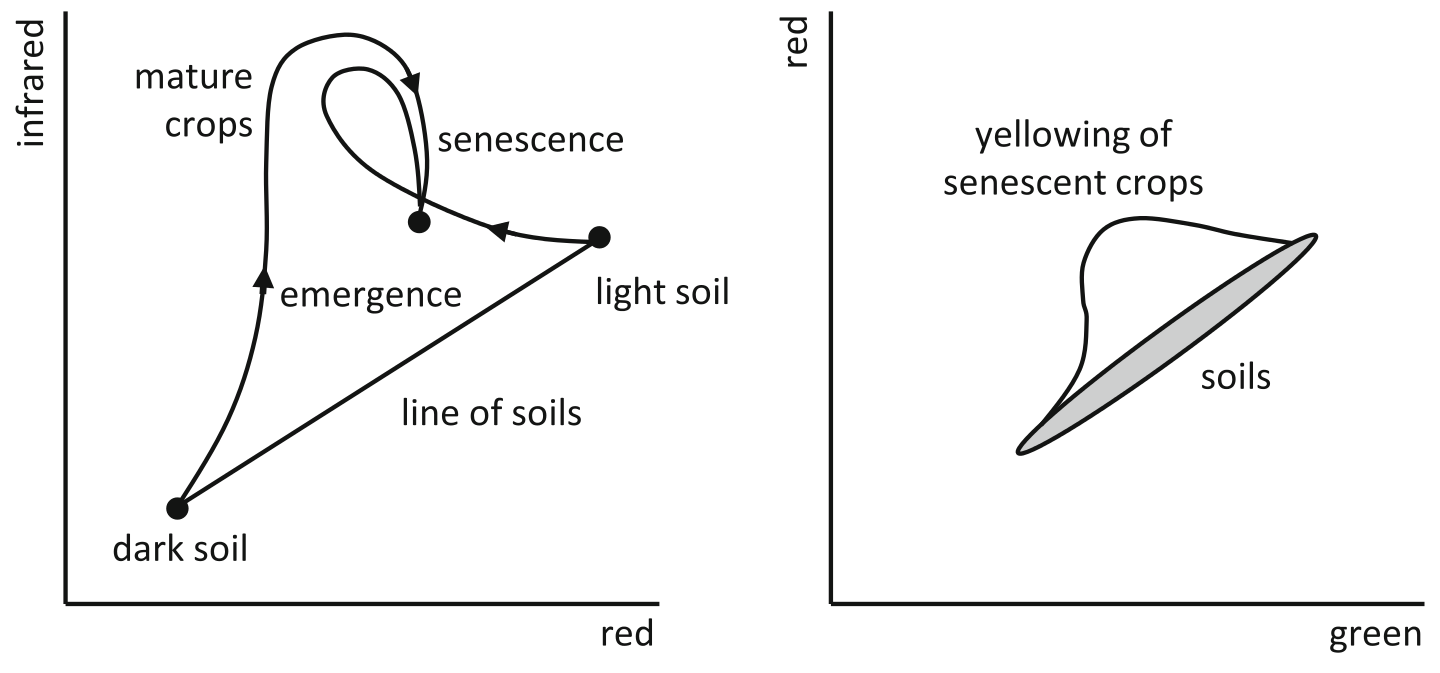
\includegraphics[width=0.8\textwidth]{imagenes/tc.png}
  \caption{Movimiento asociado al comportamiento fenológico de un píxel de vegetación en el espacio vectorial.\footfullcite{richards2013remote}}
  \end{figure}
\end{frame}
%--- Next Frame ---%


\begin{frame}{Transformada tasseled-cap}
    \begin{figure}
      \begin{tabular}{l c c c c c c }
        Combinación  & Azul & Verde & Rojo & NIR & SWIR 1 & SWIR 2\\
        Brillo &  0.30  & 0.27  & 0.47  & 0.55  & 0.50  & 0.18\\
        Verdor & -0.29  &-0.24  &-0.54  & 0.72 & 0.07  &-0.16\\
        Humedad&  0.15  & 0.19  & 0.32  & 0.34  &-0.71  &-0.45
      \end{tabular}
      \caption{Transformada tasseled-cap para landsat 8 \footfullcite{baig2014derivation}}
    \end{figure}
\end{frame}
%--- Next Frame ---%

\begin{frame}{Transformada tasseled-cap}
  \begin{block}{Idea}
    Todo esto logra hacer que el número de bandas que utilizo sea menor que el nÚmero de bandas inicial
  \end{block}
\end{frame}
%--- Next Frame ---%

\section{\'Indices}

\begin{frame}{\'Indices}
  \begin{block}{\'Indices}
    \begin{itemize}[<+>]
      \item Nos van a permitir reducir mas la dimensiónalidad.
      \item Perdiendo información.
      \item Ganando y mucho en la interpretación de los resultados.
      \item Además voy a encontrar correlaciones con variables biofísicas.
    \end{itemize}
  \end{block}
\end{frame}
%--- Next Frame ---%

\subsection{\'Indices de Vegetación}

\begin{frame}{\'Indices de Vegetación}
    \begin{figure}
    \centering
    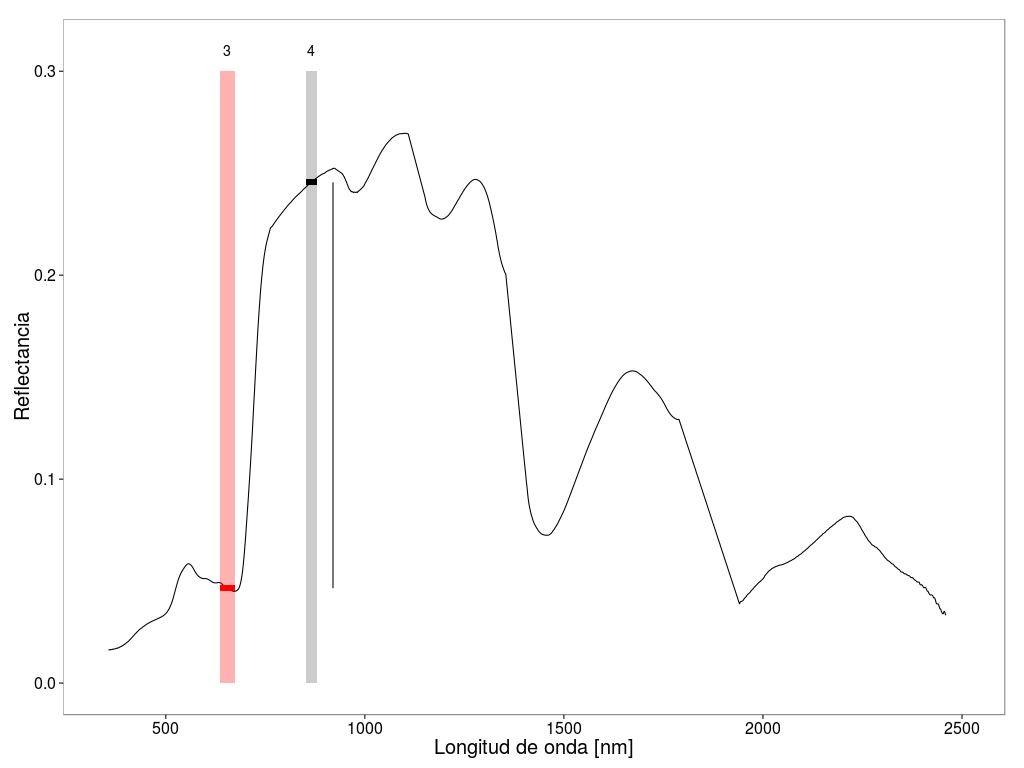
\includegraphics[width=0.8\textwidth]{imagenes/salto_nr.png}
    \caption{Salto de reflectancia entre la región entre el rojo y el infrarrojo cercano.\footfullcite{clark2007usgs}}
    \end{figure}
\end{frame}
%--- Next Frame ---%

\begin{frame}{\'Indices de Vegetación}
  \begin{block}{Definición}
    Cociente simple $$\frac{NIR}{RED}$$
    Es de lo mas sencillo que uno puede pensar.
  \end{block}
  \begin{exampleblock}{Ejemplos}
    \begin{figure}
      \begin{tabular}{l c }
        Cobertura  & $NIR/RED$\\
        Suelo & 1.57\\
        Agua & 0.51\\
        Vegetacion & 5.25
      \end{tabular}
      \caption{Valores típicos para el cociente simple}
    \end{figure}
  \end{exampleblock}
\end{frame}
%--- Next Frame ---%

\begin{frame}{\'Indices de Vegetación}
  \begin{block}{Definición}
    Cociente simple $$\frac{NIR-RED}{NIR+RED}$$
    La idea es normalizar la diferencia para simplificar la interpretación
  \end{block}
  \begin{exampleblock}{Ejemplos}
    \begin{figure}
      \begin{tabular}{l c }
        Cobertura  & $NDVI$\\
        Suelo & 0.22 \\
        Agua & -0.32 \\
        Vegetacion & 0.68
      \end{tabular}
      \caption{Valores típicos para el cociente simple}
    \end{figure}
  \end{exampleblock}
\end{frame}
%--- Next Frame ---%

\begin{frame}{\'Indices de Vegetación}
  \begin{block}{Observación}
    Se relaciona con el anterior como $$\frac{NIR/RED-1}{NIR/RED+1}$$
  \end{block}
\end{frame}
%--- Next Frame ---%

\begin{frame}{\'Indices de Vegetación}
  \begin{alertblock}{Observación}
    Este índice esta relacionado con varias variables biof\'isicas.
  \end{alertblock}
\end{frame}
%--- Next Frame ---%

\begin{frame}{\'Indices de Vegetación}
    \begin{figure}
    \centering
    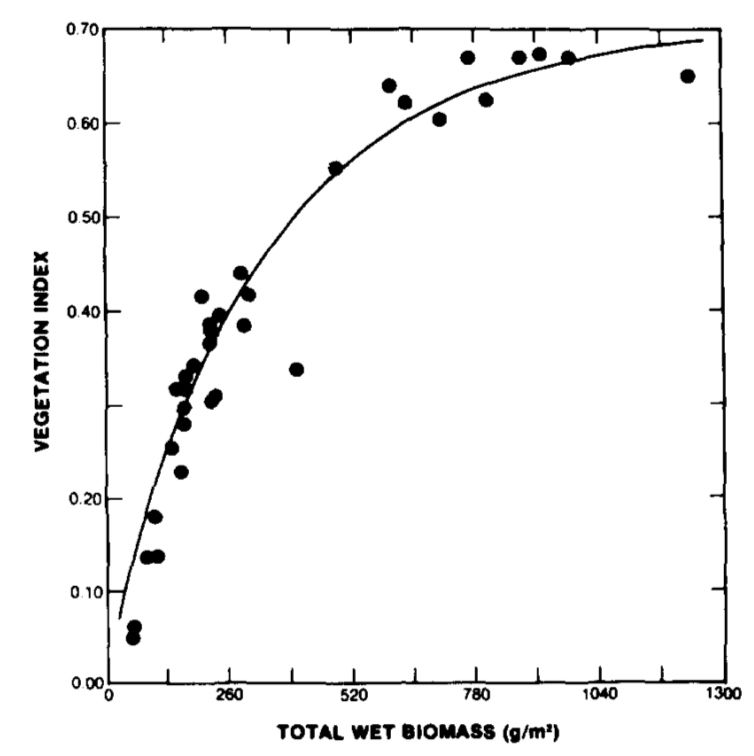
\includegraphics[width=0.6\textwidth]{imagenes/avndvi.png}
    \caption{NDVI vs cantidad de biomasa húmeda.\footfullcite{tucker1979red}}
    \end{figure}
\end{frame}
%--- Next Frame ---%

\begin{frame}{\'Indices de Vegetación}
    \begin{figure}
    \centering
    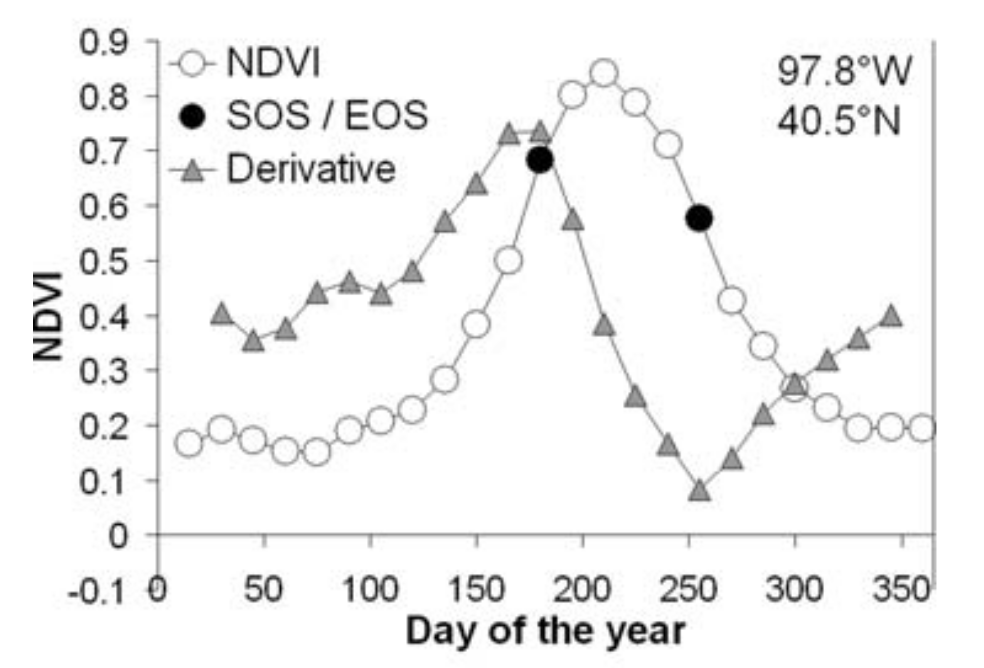
\includegraphics[width=0.8\textwidth]{imagenes/ndvivst.png}
    \caption{Variación del NDVI en función de la epoca del año.\footfullcite{de2010spatio}}
    \end{figure}
\end{frame}
%--- Next Frame ---%

\begin{frame}{\'Indices de Vegetación}
  \begin{block}{Problemas}
    \begin{itemize}[<+>]
      \item Este índice puede saturar.
      \item En suelos con baja cobertura vegetal suele ser mas difícil de interpretar.
      \item Estoy sacrificando información que puede ser relevante.
    \end{itemize}
    Por suerte hay otros índices que mejoran esta situación
  \end{block}
\end{frame}
%--- Next Frame ---%


\section{Práctica}

\begin{frame}{Práctica}
  \begin{exampleblock}{Actividades prácticas de la tercer clase}
    \begin{enumerate}
      \item Abrir imágenes Landsat 8 y digitalizar coberturas de interés.
      \item Calcular el índice de vegetación para las imágenes de febrero y agosto.
      \item Realizar curvas fenológicas a partir del índice de vegetación en la imagen MODIS.
      \item Utilizar la herramienta de componentes principales para reducir la dimensiónalidad de la imagen MODIS.
    \end{enumerate}
  \end{exampleblock}
\end{frame}
%--- Next Frame ---%

\end{document}
